  
\documentclass[letterpaper,aps,prc,superscriptaddress,nofootinbib,10pt,showpacs,floatfix]{revtex4-2}% PRC format\documentclass[12pt]
%\usepackage[super]{cite}
\usepackage{graphicx}
\usepackage{comment}
\usepackage{setspace}
\usepackage{amsmath}
\usepackage{amssymb}
%\usepackage[textwidth=16cm,textheight=22cm]{geometry}
\usepackage{color}
\usepackage{indentfirst}
\usepackage{xspace}
\usepackage{hyperref}
\usepackage{verbatim}
\usepackage{epstopdf}
\usepackage{hyperref}
\usepackage{placeins}
\usepackage{xfrac}
\usepackage[table]{xcolor}
\usepackage{array}



\newcolumntype{P}[1]{>{\centering\arraybackslash}p{#1}}
\newcolumntype{M}[1]{>{\centering\arraybackslash}m{#1}}
\newcommand{\addmathvspace}{\vrule width 0pt height 4ex depth 2.5ex}
%\usepackage{lineno}
%\RequirePackage{lineno}
%\setlength{\linenumbersep}{6pt}
%\linenumber\cite{weib1,weib2} 
\newcommand{\sqs}{\mbox{$\sqrt{s}$}\xspace}
\newcommand{\ee}{\mbox{$e^{+} e^{-}$}\xspace}
\newcommand{\pp}{\mbox{$pp\,(p\bar{p})$ }\xspace}
\newcommand{\bfrac}[2]{\frac{\displaystyle #1}{\displaystyle #2}}

\setlength{\arrayrulewidth}{0.8mm}
\graphicspath{ {./Images/} }



\begin{document}

%\titile{
%in pp collisions at 13 TeV with Pythia 8}
\title{ Measurement of higher moments of   $\cdots$}
\author{Ankan Mukherjee} 
\email{190260008@iitb.ac.in}
\affiliation{Indian Institute of Technology Bombay, Mumbai, India}
\author{YYY}
\email{XXX@iitb.ac.in}
\affiliation{Indian Institute of Technology Bombay, Mumbai, India}
\author{ZZZ}
\email{XXX@iitb.ac.in}
\affiliation{Indian Institute of Technology Bombay, Mumbai, India}

%\email{ashutosh.kumar.pandey@cern.ch}
%\email{sadhana@phy.iitb.ac.in}


\date{\today}  



\begin{abstract}

Write a proper brief abstarct ...
\end{abstract}

\maketitle

%%%%%%%%%%%%%%%%%%%%%%%%%%%%%%%%%%%%%%%%%%%%%%%%%%%%%%%%%%%%%%%%%%%%%
\section{Introduction}
%%%%%%%%%%%%%%%%%%%%%%%%%%%%%%%%%%%%%%%%%%%%%%%%%%%%%%%%%%%%%%%%%%%%%

In the ultrarelativistic nucleus to nucleus collisions, the mean transverse momentum $\mathbf{\left<p_T\right>}$, of the emitted particles fluctuates event to event.
In this project we will study these fluctuations from event to event of the $\mathbf{\left<p_T\right>}$ and plot them to study this event to event variation. 
In this project we will argue that the probability distribution of the $\mathbf{\left<p_T\right>}$, is not Gaussian but has a positive skew. 
We will also calculate \textbf{intensive skewness} and the \textbf{standard skewness} of the $\mathbf{\left<p_T\right>}$.
Also these fluctuations are not dependent on the specific set-up used in the experiment.\vspace{2mm}\\
The data provided is generated with \textbf{Pythia 8 Monte Carlo Event Generator}.\vspace{2mm}\\
Number of events :  \textbf{2 million} \\
Collisions System :  \textbf{p + p} at centre of mass energy \textbf{13 TeV}\\


%Define  the variables, moments and the used formula \\

We shall be using the \textbf{STAR definition} for our studies. The formulae used are as given below. The symbol $\left<\right>$ is used to denote the mean of the argument. $N_{ch}$ refers to the number of events corresponding to each multiplicity class.
\vspace{-5mm}
\begin{equation}
\label{eq:1}
\mathrm{Mean\ Transverse\ Momentum}=\left<\left<p_T\right>\right>=\left<\bfrac{\Sigma_{i=1}^{N_{ch}} p_i}{N_{ch}}\right>
\end{equation}
\vspace{-5mm}
\begin{equation}
\label{eq:2}
\left<\Delta p_i \Delta p_j\right>=\left<\left(\left<p_t\right>-\left<\left<p_t\right>\right>\right)^2\right>
\end{equation}
\vspace{-5mm}
\begin{equation}
\label{eq:3}
\mathrm{Intensive\ Variance\ Of\ Transverse\ Momentum}=\sigma_{p_T}=\bfrac{\left<\Delta p_i \Delta p_j\right>^{\sfrac{1}{2}}}{\left<\left<p_T\right>\right>}
\end{equation}
\vspace{-5mm}
\begin{equation}
\label{eq:4}
\left<\Delta p_i \Delta p_j \Delta p_k\right>=\left<\left(\left<p_t\right>-\left<\left<p_t\right>\right>\right)^3\right>
\end{equation}
\vspace{-5mm}
\begin{equation}
\label{eq:5}
\mathrm{Standardized\ Skewness\ Of\ Transverse\ Momentum} = \gamma_{p_T}=\bfrac{\left<\Delta p_i \Delta p_j \Delta p_k\right>}{\left<\Delta p_i \Delta p_j\right>^{\sfrac{3}{2}}}
\end{equation}
\vspace{-5mm}
\begin{equation}
\label{eq:6}
\mathrm{ Intensive\ Skewness\ Of\ Transverse\ Momentum}= 
\Gamma_{p_T}= \bfrac{\left<\Delta p_i \Delta p_j \Delta p_k\right>\left<\left<p_T\right>\right>}{\left<\Delta p_i \Delta p_j\right>^2}
\end{equation}


\section{Experimental Observations }


%1.  Distribution  of  $p_{T}$ and $<p_{T}>$ for different multiplicity classes (0-20, 20-40 etc).  \\

%All the above plots should be in logarithmic scale. \\



%2. For $|\eta < 2.5|$ (you may opt not to use any cut but mention in the text),  do the following  \\


%a.  Plot $ \sqrt{ <\Delta p_{T1} \Delta p_{T2}>} / <p_{T}> $as a function of multiplicity class. \\

%b.  Plot standardized skewness and intensive skewness as a function of multiplicity.\\

%(Use the STAR definition. Please mention if you are using any other definition.)\\

%Do not bother about errors. If possible plot the statistical errors .\\



\subsection{Transverse Momentum and Mean Transverse Momentum for Each Multiplicity Class}
In this section, we have plotted the histograms for the Transverse Momentum $\mathbf{pT}$ and the Mean Transverse Momentum $\mathbf{\left<pT\right>}$ of proton-proton collisions corresponding to each multiplicity class. The histogram for $\mathbf{pT}$ is then approximated using an \textbf{Exponential} fit, while that of $\mathbf{\left<pT\right>}$ has been approximated using a \textbf{Gaussian} fit. Both the quantities $\mathbf{pT}$ and $\mathbf{\left<pT\right>}$ have statistical fluctuations arising from the finite number of particles in each event. In each of the subsequent subsections corresponding to each of the 5 multiplicity classes, namely \hyperref[subsubsec:2040]{\textbf{pytree2040}}, \hyperref[subsubsec:4060]{\textbf{pytree4060}}, \hyperref[subsubsec:6080]{\textbf{pytree6080}}, \hyperref[subsubsec:80100]{\textbf{pytree80100}} and \hyperref[subsubsec:100]{\textbf{pytree100}}, the histograms and the corresponding fits have been plotted. A logarithmic scale has been used on the \emph{y-axis} in order to emphasize the skewness of the data. 



\subsubsection{Multiplicity Class "pytree2040"}
\label{subsubsec:2040}
\vspace{-5mm}
\begin{figure}[!htb]
   \begin{minipage}{0.48\textwidth}
   \label{Fig:1a}
   \label{Fig:1b}
     \centering
     \renewcommand{\thefigure}{1a}
     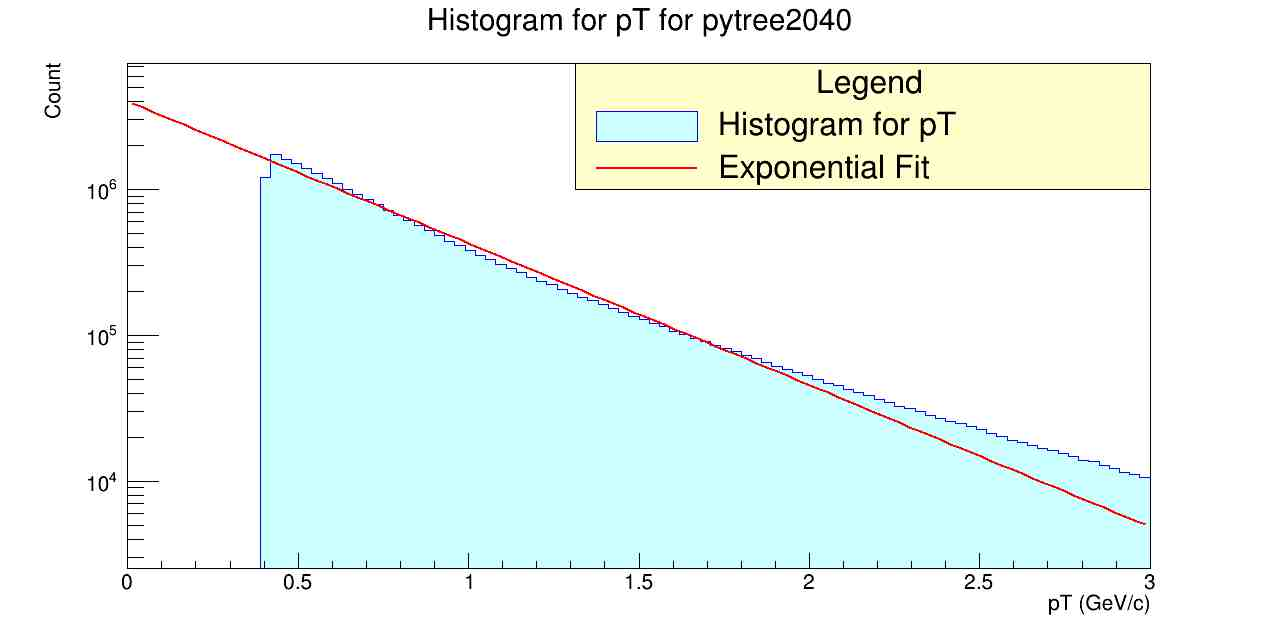
\includegraphics[width=1.1\linewidth]{pt_2040}
     \caption{(Color Online) Distribution of $\mathbf{pT}$ for proton-proton collision in the multiplicity class \textbf{pytree2040}. The solid line is an Exponential fit to the data.}
   \end{minipage}\hfill
   \begin{minipage}{0.48\textwidth}
     \centering
     \renewcommand{\thefigure}{1b}
     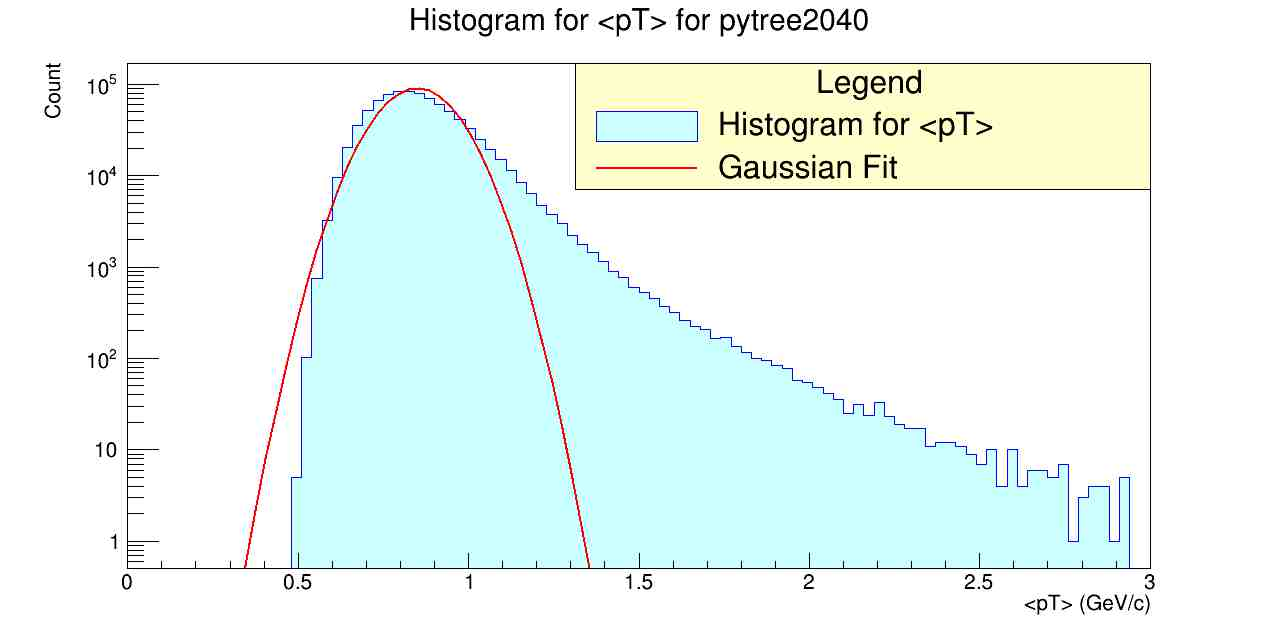
\includegraphics[width=1.1\linewidth]{/mpt_2040}
     \caption{(Color Online) Distribution of $\mathbf{\left<pT\right>}$ for proton-proton collision in the multiplicity class \textbf{pytree2040}. The solid line is a Gaussian fit to the data.}
   \end{minipage}
\end{figure}

\FloatBarrier
\vspace{-3mm}
%\pagebreak

\subsubsection{Multiplicity Class "pytree4060"}
\label{subsubsec:4060}
\vspace{-5mm}
\begin{figure}[!htb]
   \begin{minipage}{0.48\textwidth}
   \label{Fig:2a}
   \label{Fig:2b}
     \centering
     \renewcommand{\thefigure}{2a}
     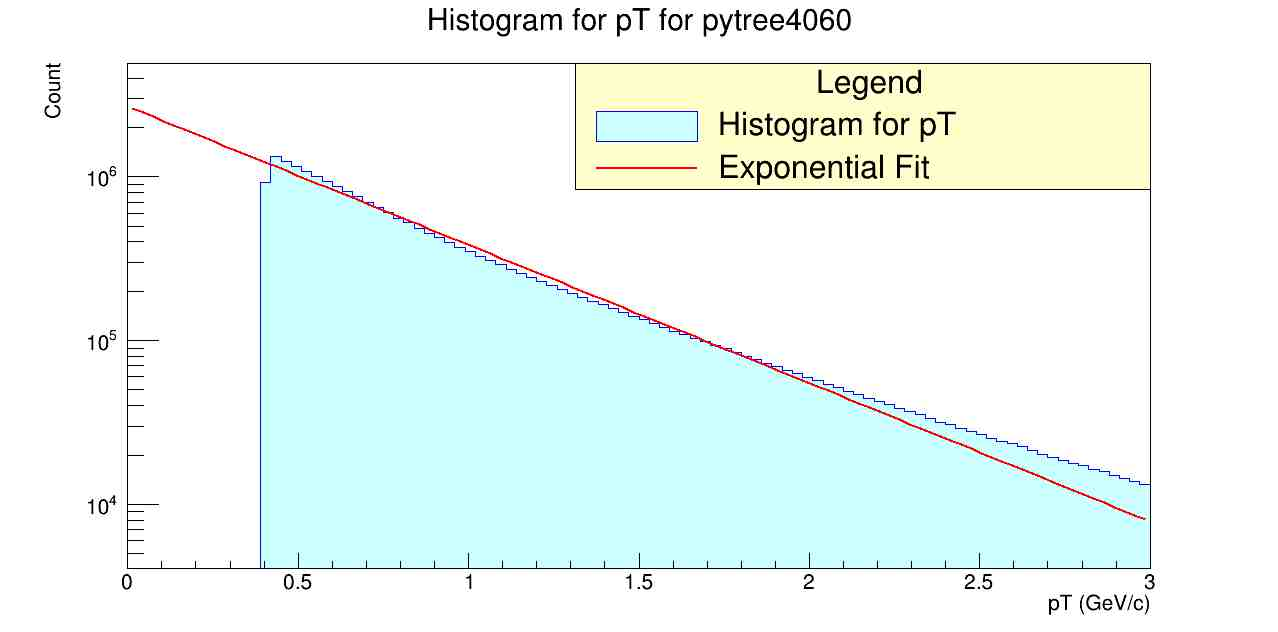
\includegraphics[width=1.1\linewidth]{pt_4060}
     \caption{(Color Online) Distribution of $\mathbf{pT}$ for proton-proton collision in the multiplicity class \textbf{pytree4060}. The solid line is an Exponential fit to the data.}
   \end{minipage}\hfill
   \begin{minipage}{0.48\textwidth}
     \centering
     \renewcommand{\thefigure}{2b}
     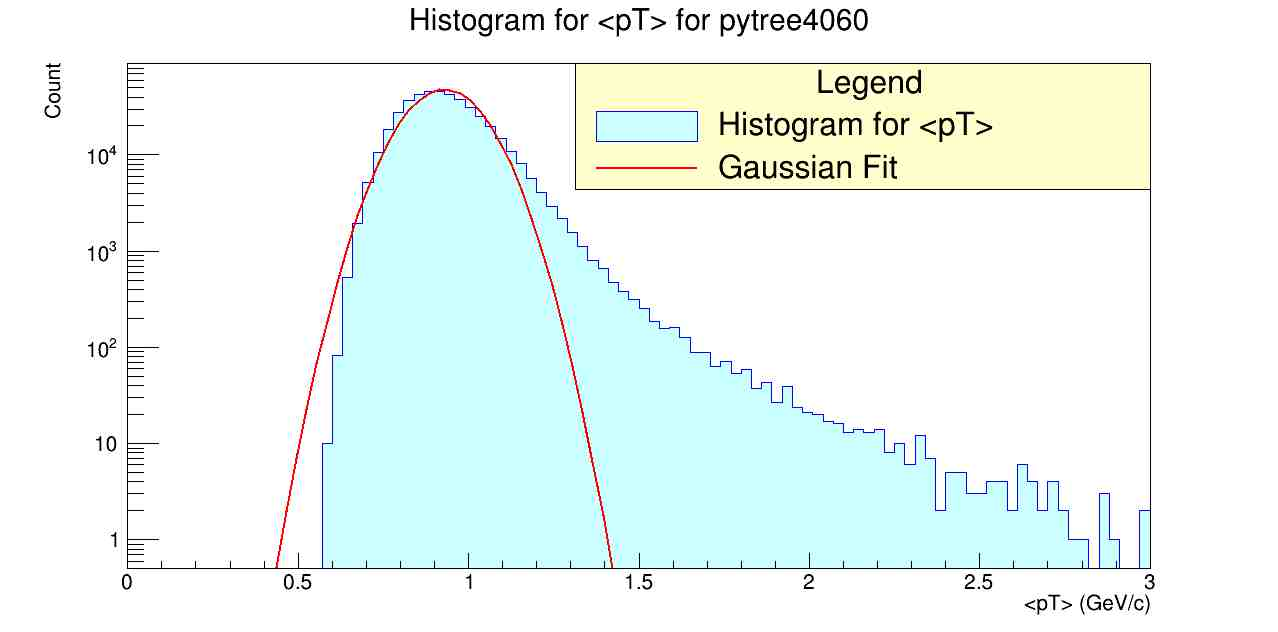
\includegraphics[width=1.1\linewidth]{/mpt_4060}
     \caption{(Color Online) Distribution of $\mathbf{\left<pT\right>}$ for proton-proton collision in the multiplicity class \textbf{pytree4060}. The solid line is a Gaussian fit to the data.}
   \end{minipage}
\end{figure}

\FloatBarrier
\vspace{-3mm}

\subsubsection{Multiplicity Class "pytree6080"}
\label{subsubsec:6080}
\vspace{-5mm}
\begin{figure}[!htb]
   \begin{minipage}{0.48\textwidth}
   \label{Fig:3a}
   \label{Fig:3b}
     \centering
     \renewcommand{\thefigure}{3a}
     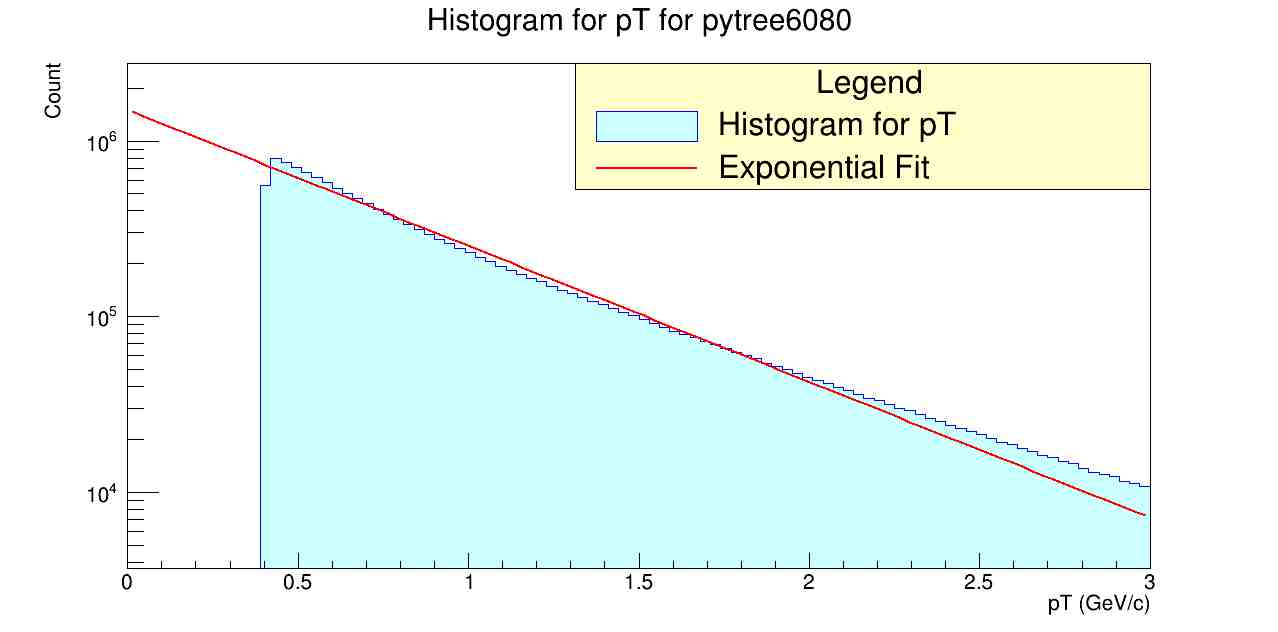
\includegraphics[width=1.1\linewidth]{pt_6080}
     \caption{(Color Online) Distribution of $\mathbf{pT}$ for proton-proton collision in the multiplicity class \textbf{pytree6080}. The solid line is an Exponential fit to the data.}
   \end{minipage}\hfill
   \begin{minipage}{0.48\textwidth}
     \centering
     \renewcommand{\thefigure}{3b}
     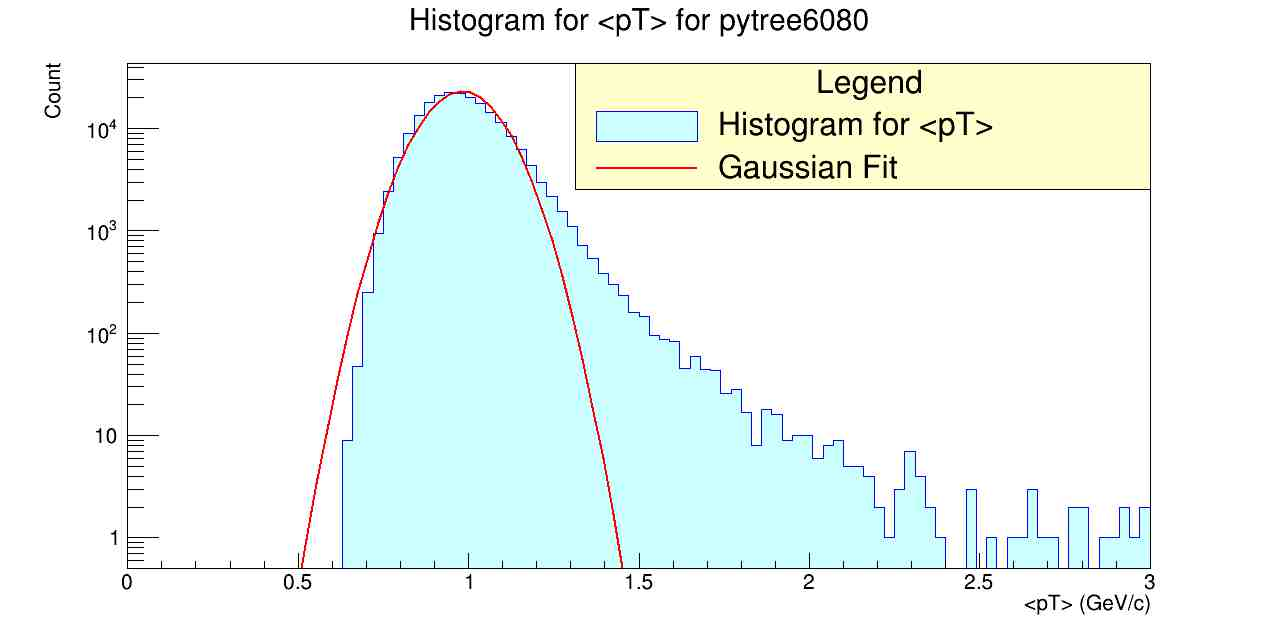
\includegraphics[width=1.1\linewidth]{/mpt_6080}
     \caption{(Color Online) Distribution of $\mathbf{\left<pT\right>}$ for proton-proton collision in the multiplicity class \textbf{pytree6080}. The solid line is a Gaussian fit to the data.}
   \end{minipage}
\end{figure}

\FloatBarrier
\vspace{-3mm}

\subsubsection{Multiplicity Class "pytree80100"}
\label{subsubsec:80100}
\vspace{-5mm}
\begin{figure}[!htb]
   \begin{minipage}{0.48\textwidth}
   \label{Fig:4a}
   \label{Fig:4b}
     \centering
     \renewcommand{\thefigure}{4a}
     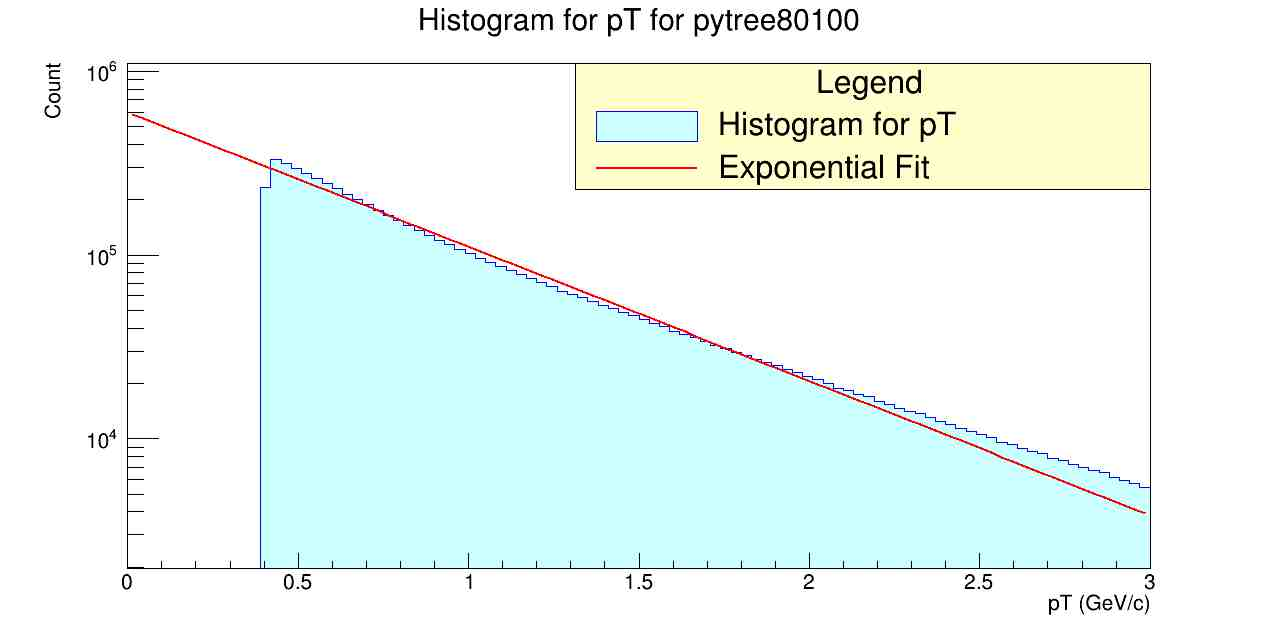
\includegraphics[width=1.1\linewidth]{pt_80100}
     \caption{(Color Online) Distribution of $\mathbf{pT}$ for proton-proton collision in the multiplicity class \textbf{pytree80100}. The solid line is an Exponential fit to the data.}
   \end{minipage}\hfill
   \begin{minipage}{0.48\textwidth}
     \centering
     \renewcommand{\thefigure}{4b}
     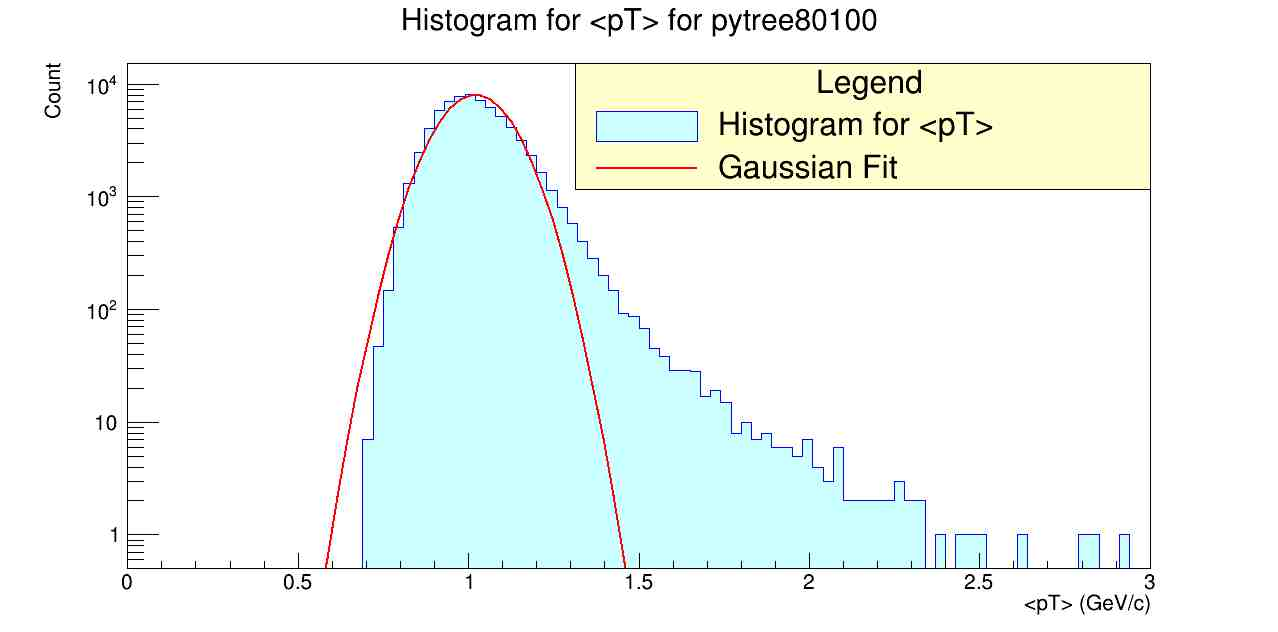
\includegraphics[width=1.1\linewidth]{/mpt_80100}
     \caption{(Color Online) Distribution of $\mathbf{\left<pT\right>}$ for proton-proton collision in the multiplicity class \textbf{pytree80100}. The solid line is a Gaussian fit to the data.}
   \end{minipage}
\end{figure}

\FloatBarrier
\vspace{-3mm}

\subsubsection{Multiplicity Class "pytree100"}
\label{subsubsec:100}
\vspace{-5mm}
\begin{figure}[!htb]
   \begin{minipage}{0.48\textwidth}
   \label{Fig:5a}
   \label{Fig:5b}
     \centering
     \renewcommand{\thefigure}{5a}
     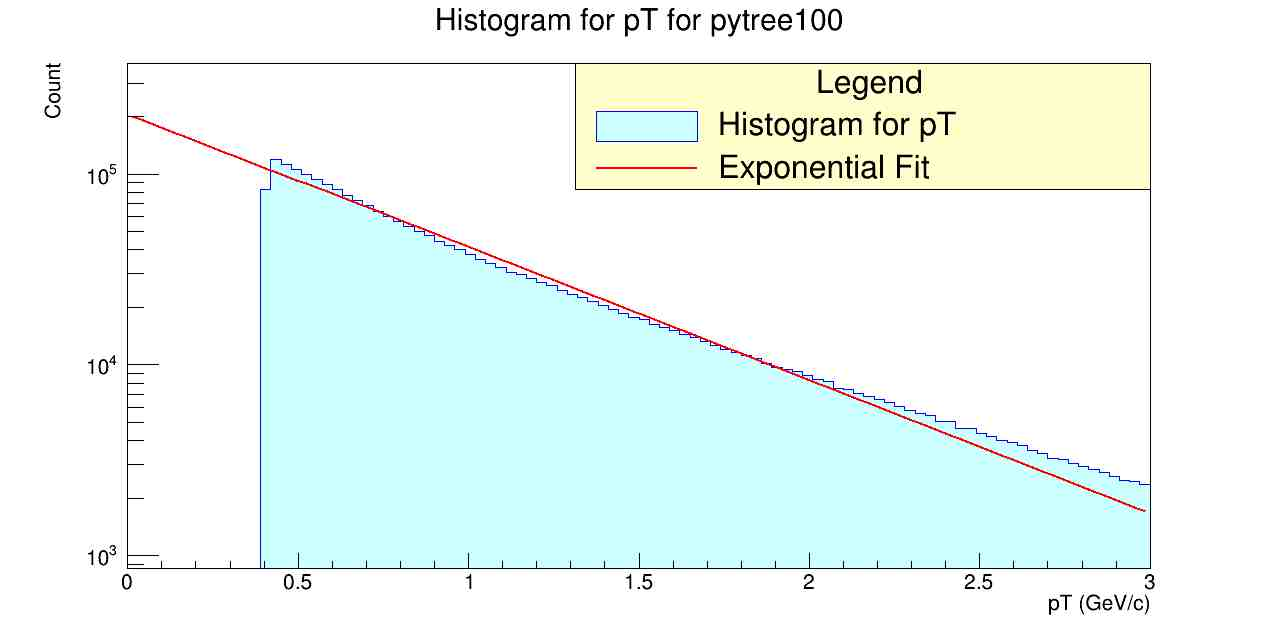
\includegraphics[width=1.1\linewidth]{pt_100}
     \caption{(Color Online) Distribution of $\mathbf{pT}$ for proton-proton collision in the multiplicity class \textbf{pytree100}. The solid line is an Exponential fit to the data.}
   \end{minipage}\hfill
   \begin{minipage}{0.48\textwidth}
     \centering
     \renewcommand{\thefigure}{5b}
     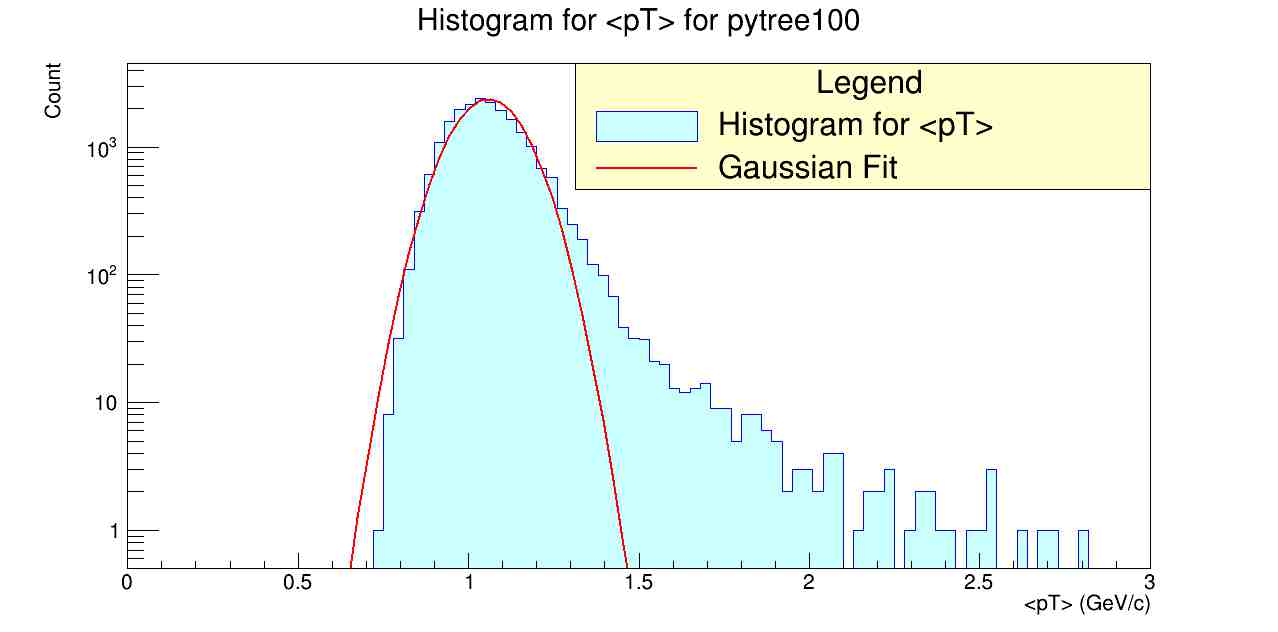
\includegraphics[width=1.1\linewidth]{/mpt_100}
     \caption{(Color Online) Distribution of $\mathbf{\left<pT\right>}$ for proton-proton collision in the multiplicity class \textbf{pytree100}. The solid line is a Gaussian fit to the data.}
   \end{minipage}
\end{figure}

\FloatBarrier

\subsection{Analysis of Mean, Variance and Skewness Versus Multiplicity Class}
From the graphs in \hyperref[Fig:1a]{FIG. 1a.}, \hyperref[Fig:2a]{FIG. 2a.}, \hyperref[Fig:3a]{FIG. 3a.}, \hyperref[Fig:4a]{FIG. 4a.} and \hyperref[Fig:5a]{FIG. 5a.}, it is clear that the Transverse Momenta of the particles produced in a proton-proton collision follows approximately an \textbf{exponential distribution}. Graphs in \hyperref[Fig:1b]{FIG. 1b.}, \hyperref[Fig:2b]{FIG. 2b.}, \hyperref[Fig:3b]{FIG. 3b.}, \hyperref[Fig:4b]{FIG. 4b.} and \hyperref[Fig:5b]{FIG. 5b.} reveal that there is some \textbf{positive skew} in the distribution of the Mean Transverse Momentum.
\\
In this section, we shall analyse the moments of the distribution of Transverse Momentum. We shall calculate the Mean, Variance and Skewness of the Transverse Momenta for each multiplicity class and study its relation with the multiplicity class. For each of the multiplicity classes, the Mean Transverse Momentum, the Intensive Variance of the Transverse Momentum, the Standardized Skewness of the Transverse Momentum and the Intensive Skewness of the Transverse Momentum, calculated using formulae \ref{eq:1}, \ref{eq:3} respectively have been summarised in the \hyperref[subsubsec:summary]{table} and the \hyperref[subsubsec:mean]{plots} below.

%\pagebreak
\newpage

\subsubsection{Summary of Data}
\label{subsubsec:summary}
\vspace{-5mm}
The table below summarizes the data.
\begin{table}[!htb]
\centering
	\begin{tabular}{|M{5cm}|M{2cm}|M{2cm}|M{2cm}|M{2cm}|M{2cm}|}
		\hline
		\multicolumn{6}{|c|}{\addmathvspace\textbf{SUMMARY OF DATA}}\\
		\hline
		\addmathvspace\textbf{Multiplicity Class} & 
		$\mathbf{Events}$ & 
		\begin{tabular}{c}
			$\large\mathbf{\left<p_T\right>}$\\[2pt]
			\textbf{(GeV/c)}
		\end{tabular} &
		$\large\mathbf{\sigma_{p_T}}$ & 
		\begin{tabular}{c}
			$\large\mathbf{\gamma_{p_T}}$\\[2pt]
			\textbf{(GeV/c)}
		\end{tabular} &		 
		$\large\mathbf{\Gamma_{p_T}}$\\[10pt]
		\hline
		\textit{pytree2040}&\addmathvspace873322&0.869307&0.174974&1.77742&10.1582\\[5pt]
		\hline
		\textit{pytree4060}&\addmathvspace445805&0.940521&0.144591&1.80884&12.51\\[5pt]
		\hline
		\textit{pytree6080}&\addmathvspace207990&0.99074&0.130471&3.11451&23.8714\\[5pt]
		\hline
		\textit{pytree80100}&\addmathvspace71263&1.03006&0.122603&1.64507&13.4178\\[5pt]
		\hline
		\textit{pytree100}&\addmathvspace20981&1.07257&0.132207&4.11805&31.1485\\[5pt]
		\hline		
	\end{tabular}
	\caption{Table Summarizing the Data of Transverse Momenta}
\end{table}

\FloatBarrier

\subsubsection{Mean Transverse Momentum versus Multiplicity Class}
\label{subsubsec:mean}
\vspace{-5mm}
\begin{figure}[!htb]
	\begin{minipage}{0.9\textwidth}
   		\label{Fig:6}
     	\centering
     	\renewcommand{\thefigure}{6}
     	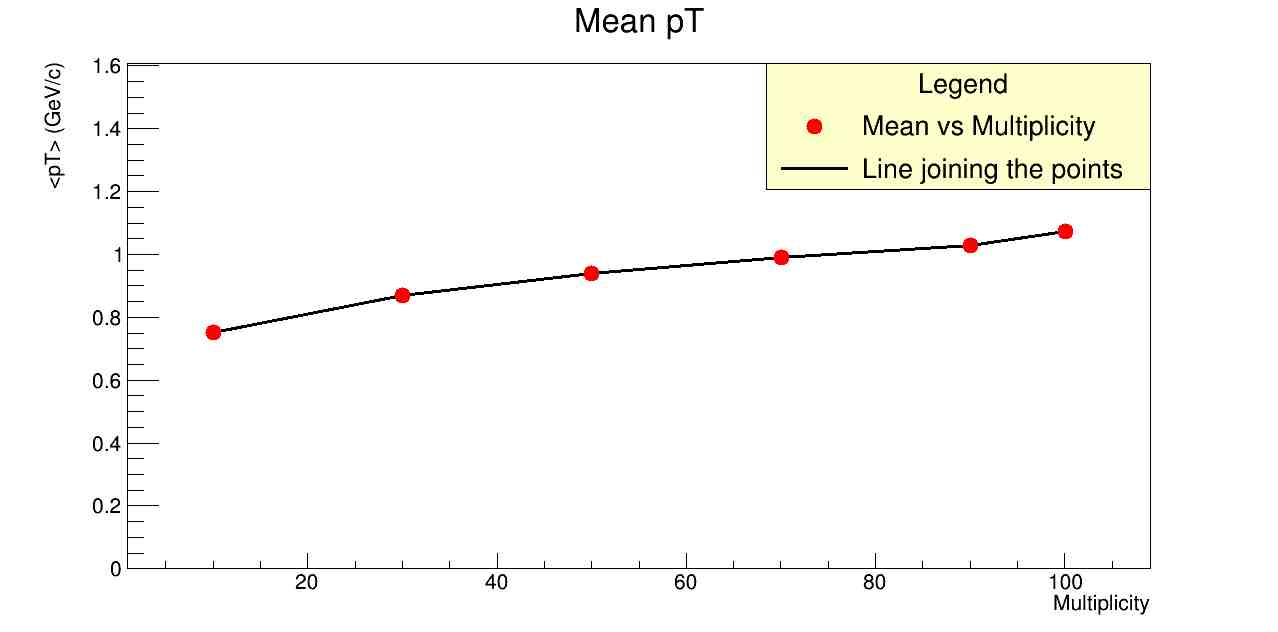
\includegraphics[width=0.9\linewidth]{mean}
     	\caption{(Color Online) A plot of \textbf{mean} transverse momenta versus multiplicity class. The red dots represent the mean of the transverse momentum. The solid line shows the trend of the mean against the multiplicity class.}
     \end{minipage}
\end{figure}

\FloatBarrier
\vspace{-3mm}
\pagebreak


\subsubsection{Intensive Variance of Transverse Momentum versus Multiplicity Class}
\label{subsubsec:intvar}
\vspace{-5mm}
\begin{figure}[!htb]
\begin{minipage}{0.9\textwidth}
   \label{Fig:7}
     \centering
     \renewcommand{\thefigure}{7}
     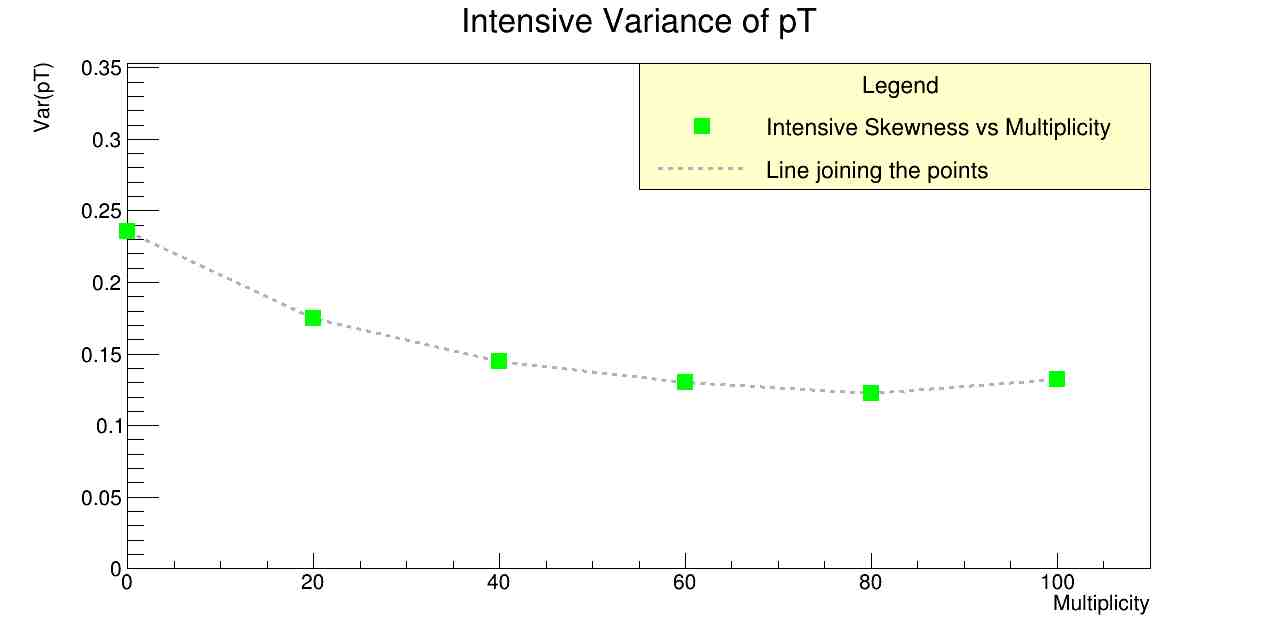
\includegraphics[width=0.9\linewidth]{intvar}
     \caption{(Color Online) A plot of the \textbf{intensive variance} of transverse momenta versus multiplicity class. The green boxes represent the intensive variance of the transverse momentum. The dashed line shows the trend of the intensive variance against the multiplicity class.}
\end{minipage}
\end{figure}

\FloatBarrier
\vspace{-3mm}

\subsubsection{Standardized Skewness of Transverse Momentum versus Multiplicity Class}
\label{subsubsec:stdskew}
\vspace{-5mm}
\begin{figure}[!htb]
\begin{minipage}{0.9\textwidth}
   \label{Fig:8}
     \centering
     \renewcommand{\thefigure}{8}
     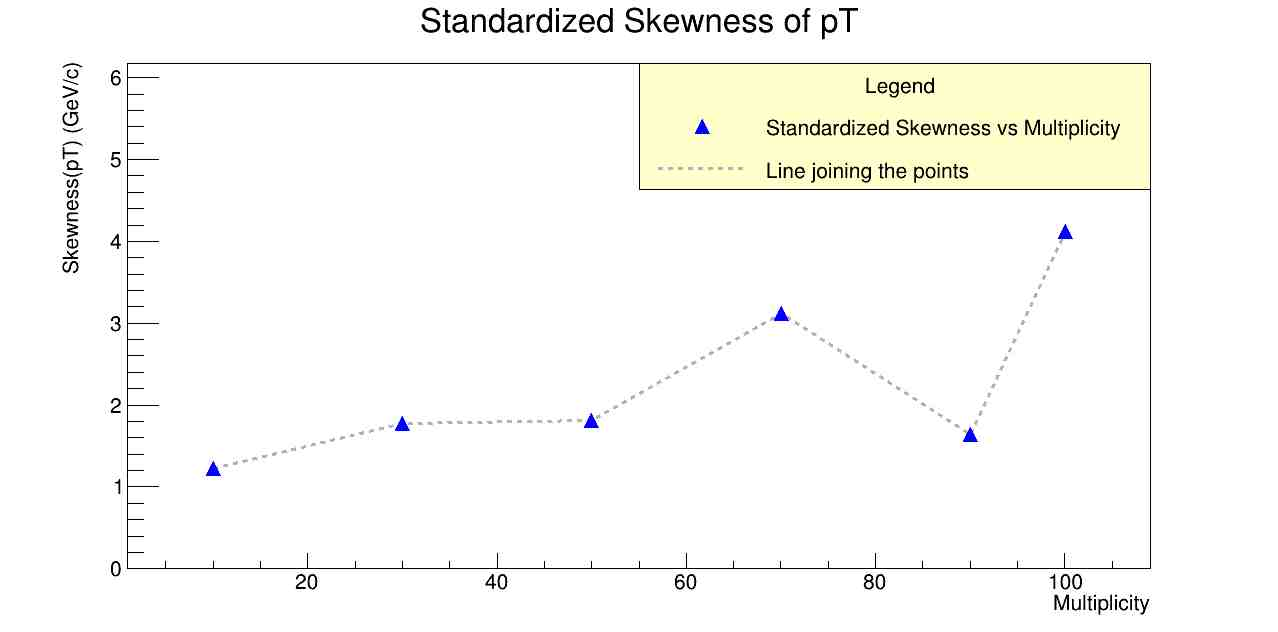
\includegraphics[width=0.9\linewidth]{stdskew}
     \caption{(Color Online) A plot of the \textbf{standardized skewness} of transverse momenta versus multiplicity class. The blue triangles represent the standardized skewness of the transverse momentum. The dashed line shows the trend of the standardized skewness against the multiplicity class.}
\end{minipage}
\end{figure}

\FloatBarrier
\vspace{-1mm}
\pagebreak

\subsubsection{Intensive Skewness of Transverse Momentum versus Multiplicity Class}
\label{subsubsec:intskew}
\vspace{-5mm}
\begin{figure}[!htb]
\begin{minipage}{0.9\textwidth}
   \label{Fig:9}
     \centering
     \renewcommand{\thefigure}{9}
     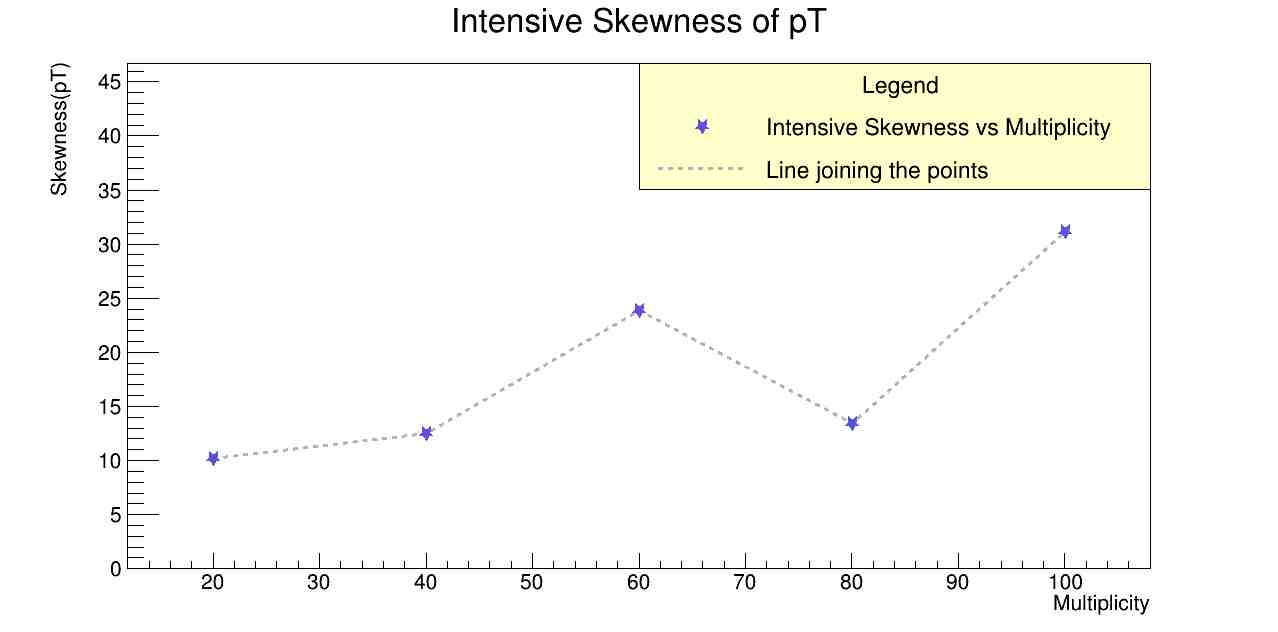
\includegraphics[width=0.9\linewidth]{intskew}
     \caption{(Color Online) A plot of the \textbf{intensive skewness} of transverse momenta versus multiplicity class. The cyan stars represent the intensive skewness of the transverse momentum. The dashed line shows the trend of the intensive skewness against the multiplicity class.}
\end{minipage}
\end{figure}










\newpage
\begin{figure*}
\begin{center}
%\includegraphics[scale=0.8]{ppspectra.eps}
\caption{(Color online) Put proper captions}
\label{f1}
\end{center}
\end{figure*}









\section{Summary}

The study of  $\cdots$


\begin{thebibliography}{50}
\medskip


%\bibitem{phenixwhite} K. ~Adcox 
  %Nuclear Phys. A{\bf 757},184-283 (2005). 
  
\bibitem{alicenature} J. ~Adams {\it et al.}, (ALICE Collaboration), Nature Physics{\bf 13},535-539 (2017). 


\end{thebibliography}

\end{document}

